% Provenance (never printed): see sources/outline_sources.md (Year 3: gravity, magnetic,
% seismic, resistivity and ground-penetrating-radar surveys; data processing and
% uncertainty; a mapping project).
% Brief: sources/book5/BRIEFS.md, ch. 31. Curves from figdata/bachelor-3/gravity_granite.py
% (prism model of the Varden granite of figdata/shared/region.py), magnetic_dyke.py (2-D
% dyke; the Varden dolerite dyke of the Sync 3 ruling, buried below the unconformity),
% resistivity_sounding.py (Pekeris transform and image series) and gpr_radargram.py.
% Physical-property ranges and survey practice from the GPG open textbook (CC BY 4.0) and
% Keys (1990). Exercise and problem values in the Book 5 scratch calculator calc/ch31.py.
\chapter{Metode Lapangan dan Laboratorium III}\label{ch:b3:field-lab-methods-3}

Sebuah tim geofisika menghabiskan satu minggu di lembah Perbukitan Varden,
wilayah fiktif yang peta geologinya digambarkan oleh volume Tahun~1 dalam
bab tentang peta geologi. Peta itu menunjukkan granit yang tersingkap di
lereng lembah, di antara sekis, di bawah batu pasir yang
bertumpu di atas keduanya. Di mana granit masuk di bawah penutup, seberapa jauh ia
membentang dan seberapa dalam ia mencapai, tidak seorang pun pernah melihatnya. Tim membawa sebuah
gravimeter, dua magnetometer, kabel elektrode, dan radar di atas
gerobak kecil. Tidak satu pun dari instrumen ini melihat batuan: masing-masing mengukur
medan di permukaan---gravitasi, medan magnet, potensial listrik,
gema denyut radio---yang diganggu batuan di bawahnya.
Pada akhir minggu, tim dapat menggambar granit yang tidak pernah mereka lihat, menyebutkan
seberapa dalam aluvium dasar lembah, dan melaporkan sebuah benda magnetik
yang tidak ditunjukkan peta mana pun.

Bab ini mengikuti minggu itu. Setiap metode dibahas satu per satu, sebagai
pengukuran beserta koreksinya dan sebagai \omterm{def:b3:seismology-imaging:inverse}{masalah maju} dengan beberapa
benda yang medannya dapat dihitung secara eksak; setelah itu dijelaskan bagaimana
kesalahan suatu survei terakumulasi dan mengapa satu jenis data jarang menentukan
model; bab ini diakhiri dengan survei Varden, tempat metode-metode itu
dipadukan.

\begin{recall}
Anomali gravitasi, koreksi dan anomali udara-bebas serta Bouguer, dan
gravitasi normal terdapat dalam volume Tahun~1, pada bab tentang isostasi
dan gravitasi; loop survei \omterm{def:b3:field-lab-methods-3:gravimeter}{gravimeter relatif} dijelaskan dalam
\cref{ch:b3:gravity-geodesy}. Medan utama, inklinasinya, \omterm{thm:b3:palaeomagnetism:dipole}{rumus
dipol} dan \omterm{def:b3:palaeomagnetism:igrf}{medan referensi geomagnetik internasional} dibahas dalam
\cref{ch:b3:palaeomagnetism}. Resistivitas, hukum Ohm, permitivitas
relatif, gelombang elektromagnetik, magnetisasi dan
suseptibilitas magnetik ada di buku fisika, dan teorema Gauss untuk
gravitasi, juga di sana. \omterm{def:b3:exploration-seismology:surveys}{Survei refraksi seismik} dibahas dalam
\cref{ch:b3:exploration-seismology}; \omterm{def:b3:seismology-imaging:inverse}{masalah maju} dan \omterm{def:b3:seismology-imaging:inverse}{masalah invers} serta
kuadrat terkecil berbobot dalam \cref{ch:b3:seismology-imaging}; porositas dalam
buku sekolah dan \omterm{def:b3:facies-models:wireline}{log kabel} dalam \cref{ch:b3:facies-models}. Perambatan
ketidakpastian dibahas dalam buku kimia dan buku matematika.
\end{recall}

\section{Survei gravitasi}\label{sec:b3:field-lab-methods-3:gravity}

Anomali yang dicari survei gravitasi berukuran kecil. Gravitasi di
khatulistiwa sekitar \qty{978000}{\milli\gal}; struktur besar mengubahnya
hingga ratusan miligal, kubah garam sekitar sepuluh, badan bijih sekitar
satu, dan target survei geoteknik sekitar beberapa
perseratus. Geofisikawan mengukur dalam
miligal, atau dalam satuan gravitasi \qty{0.1}{\milli\gal}; survei yang berguna
harus mampu membedakan selisih satu per seratus juta dari~$g$.
% ledger: gpg:grav-units, gpg:grav-sizes

\begin{definition}[Gravimeter relatif; hanyutan instrumen]\label{def:b3:field-lab-methods-3:gravimeter}
Sebuah \emph{gravimeter relatif}\index{gravimeter relatif} adalah
instrumen yang mengukur selisih gravitasi antarstasiun: sebuah
massa pada pegas, dijaga pada posisi nol oleh gaya kedua yang dapat diatur
yang pembacaan skalanya, dikalikan konstanta kalibrasi, memberikan gravitasi
dalam miligal hingga suatu konstanta tak diketahui. Yang disebut \emph{hanyutan
instrumen}\index{hanyutan instrumen} adalah perubahan lambat pembacaannya pada
stasiun tetap, disebabkan oleh rayapan pegas, suhu dan
guncangan; ia diukur dengan membaca ulang, setelah beberapa jam, stasiun
yang sudah dibaca, yakni \emph{stasiun basis}.
\end{definition}
% ledger: gpg:gravimeter, gpg:grav-survey

Gravimeter lapangan mencakup rentang beberapa puluh ribu
miligal dan membaca, pada kondisi terbaiknya, hingga sekitar \qty{0.01}{\milli\gal}; rentang
harus diatur ulang setelah diangkut. Pada ketelitian itu, tinggi
setiap stasiun sama pentingnya dengan pembacaannya: kesalahan tinggi
sebesar \qty{3.3}{cm} sudah merusak \qty{0.01}{\milli\gal}, sehingga posisi diukur
dengan penerima satelit atau waterpas hingga sentimeter. Stasiun basis
dikunjungi ulang setiap beberapa jam. Pasang surut bumi padat, yang dapat
mencapai \qty{0.3}{\milli\gal}, berubah cukup lambat selama jam-jam tersebut
sehingga dapat dihilangkan bersama hanyutan.
% ledger: gpg:gravimeter, gpg:grav-survey, gpg:grav-sizes

\begin{method}[Mereduksi loop gravitasi]\label{met:b3:field-lab-methods-3:loop}
Sebuah loop dimulai dan berakhir di stasiun basis, dibaca pada waktu $t_0$ dan $t_1$.
\begin{enumerate}
  \item Hitung laju hanyutan $(r_1 - r_0)/(t_1 - t_0)$ dari kedua
        pembacaan basis; laju ini sudah mencakup pasang surut.
  \item Kurangkan dari setiap pembacaan hanyutan yang terakumulasi sejak $t_0$,
        $r - (t - t_0)(r_1 - r_0)/(t_1 - t_0)$, dan kurangkan
        pembacaan basis: ini adalah gravitasi relatif terhadap basis.
  \item Koreksi untuk tinggi $\Delta h$ stasiun di atas basis:
        tambahkan koreksi udara-bebas $\qty{0.3086}{\milli\gal.m^{-1}}
        \times\Delta h$ dan kurangkan koreksi Bouguer
        $\qty{0.1119}{\milli\gal.m^{-1}}\times\Delta h$ (massa jenis
        \qty{2670}{kg.m^{-3}}), yakni tambahkan $0.1967\,\Delta h$.
  \item Untuk stasiun yang berjarak $\Delta y$ ke utara dari basis, kurangkan
        perubahan gravitasi normal, $\qty{0.811}{\milli\gal.km^{-1}}
        \times\sin 2\varphi\times\Delta y$.
  \item Tambahkan \omterm{def:b3:field-lab-methods-3:terrain}{koreksi medan} setiap stasiun.
\end{enumerate}
Hasilnya adalah anomali Bouguer relatif terhadap basis. Dengan mengikatkan basis
ke stasiun yang gravitasi mutlaknya diketahui, diperoleh anomali itu sendiri.
\end{method}
% ledger: gpg:grav-survey, gpg:terrain

Koreksi Bouguer memperlakukan tanah di antara stasiun dan
bidang acuan sebagai lempengan datar. Pada relief nyata, ini keliru dua kali:
bukit yang menjulang di atas stasiun menarik ke atas dan menurunkan
pembacaan, dan lembah yang turun di bawahnya dihitung dalam lempengan sebagai
batuan yang sebenarnya tidak ada.

\begin{definition}[Koreksi medan]\label{def:b3:field-lab-methods-3:terrain}
Yang disebut \emph{koreksi medan}\index{koreksi medan} di suatu stasiun gravitasi
adalah tarikan yang diberikan oleh penyimpangan relief dari
lempengan Bouguer terhadap stasiun itu: bukit di atas ketinggian stasiun, dan
lembah di bawahnya, dihitung dengan massa jenis lempengan.
Keduanya menurunkan gravitasi terukur dibanding lempengan, sehingga koreksinya
selalu ditambahkan.
\end{definition}

Dahulu dihitung dengan tangan, memakai bagan Hammer dan tabel, zona demi zona
menjauhi stasiun; kini dihitung dari sebuah model elevasi
digital. Jauh dari relief curam, nilainya jarang melebihi \qty{1}{\milli\gal},
tetapi zona-zona yang dekat dengan stasiun sulit dihitung dengan benar, dan
koreksinya jarang diketahui lebih teliti dari \qty{0.2}{\milli\gal}.
% ledger: gpg:terrain, gpg:grav-sizes

\subsection{Anomali benda sederhana}

\omterm{def:b3:seismology-imaging:inverse}{Masalah maju} gravitasi adalah sebuah penjumlahan: setiap elemen benda
dengan kontras massa jenis $\Delta\rho$ menarik stasiun menurut hukum Newton, dan
survei mengukur komponen vertikal dari penjumlahan itu. Beberapa benda memberinya
dalam bentuk tertutup.

\begin{theorem}[Bola dan silinder horizontal]\label{thm:b3:field-lab-methods-3:sphere}
Pada jarak horizontal $x$ dari titik tepat di atas pusatnya, sebuah bola
terkubur dengan kelebihan massa $\Delta m$ yang pusatnya pada kedalaman $z$ memberikan
anomali
\[
\Delta g(x) = \frac{G\,\Delta m\,z}{(x^2 + z^2)^{3/2}} ,
\]
dan anomali turun menjadi setengah dari puncaknya pada $x_{1/2} = z\sqrt{2^{2/3} - 1}$,
sehingga $z = 1.305\,x_{1/2}$. Silinder horizontal panjang dengan kelebihan massa
$\lambda$ per satuan panjang dan sumbunya pada kedalaman $z$, memberikan
anomali tegak lurus jurusnya
\[
\Delta g(x) = \frac{2G\lambda z}{x^2 + z^2} ,
\]
dan $z = x_{1/2}$.
\end{theorem}

\begin{proof}
Di luar bola yang massa jenisnya hanya bergantung pada jarak dari
pusatnya, tarikannya sama dengan tarikan massa yang diletakkan di pusat (teorema
cangkang, akibat dari teorema Gauss). Besarnya di
stasiun adalah $G\Delta m/(x^2 + z^2)$, dan komponen vertikalnya memuat
faktor $z/\sqrt{x^2 + z^2}$. Dengan menuliskan $\Delta g(x_{1/2}) =
\Delta g(0)/2$ diperoleh $(1 + x_{1/2}^2/z^2)^{3/2} = 2$, maka aturan itu. Untuk
silinder, teorema Gauss pada silinder koaksial berjari-jari $r$ memberikan
medan $2G\lambda/r$, dan komponen vertikalnya $2G\lambda z/r^2$;
setengah puncak tercapai ketika $x^2 + z^2 = 2z^2$.
\end{proof}
% ledger: gpg:half-width

Benda yang bukan bola tetap memiliki lebar setengah puncak, dan aturan itu
memberikan kedalaman bola setara, bukan kedalaman bendanya. Aturan itu
hanyalah tebakan awal, dibuat sebelum model apa pun dicocokkan.

\begin{proposition}[Silinder vertikal pada sumbunya]\label{prop:b3:field-lab-methods-3:vcyl}
Silinder vertikal berjari-jari $a$ dan kontras massa jenis $\Delta\rho$,
dengan puncak dan dasarnya pada kedalaman $z_1 < z_2$ di bawah stasiun,
memberikan pada sumbunya
\[
\Delta g = 2\pi G\Delta\rho\left[(z_2 - z_1) + \sqrt{z_1^2 + a^2}
           - \sqrt{z_2^2 + a^2}\right] .
\]
Untuk $a \to \infty$ ini menjadi lempengan Bouguer $2\pi G\Delta\rho(z_2 - z_1)$;
untuk silinder dari permukaan hingga kedalaman besar, nilainya cenderung
menuju $2\pi G\Delta\rho\,a$.
\end{proposition}

\begin{proof}
Cakram berjari-jari $a$ dan tebal $\mathrm{d}z$ pada kedalaman $z$ menarik
titik pada sumbunya sebesar $2\pi G\Delta\rho\,\mathrm{d}z\,(1 -
z/\sqrt{z^2 + a^2})$, yaitu tarikan cincin yang diintegralkan terhadap
jari-jari. Mengintegralkan dari $z_1$ ke $z_2$ menghasilkan kurung. Ketika $a \to
\infty$ pada kedalaman tetap, $\sqrt{z_1^2 + a^2} - \sqrt{z_2^2 + a^2} =
(z_1^2 - z_2^2)/(\sqrt{z_1^2 + a^2} + \sqrt{z_2^2 + a^2}) \to 0$; ketika
$z_1 = 0$ dan $z_2 \to \infty$, $z_2 - \sqrt{z_2^2 + a^2} \to 0$ dan
kurung cenderung ke $a$.
\end{proof}

\begin{proposition}[Kelebihan massa dari peta gravitasi]\label{prop:b3:field-lab-methods-3:gauss}
Berapa pun bentuk benda yang seluruhnya terletak di bawah bidang
horizontal, kelebihan massanya adalah
\[
\Delta m = \frac{1}{2\pi G}\iint \Delta g\,\mathrm{d}A ,
\]
dengan integral meliputi seluruh bidang.
\end{proposition}

\begin{proof}
Untuk massa titik $m$ pada kedalaman $z$, dengan $r$ jarak horizontal,
$\iint \Delta g\,\mathrm{d}A = \int_0^\infty
Gmz\,(r^2 + z^2)^{-3/2}\,2\pi r\,\mathrm{d}r = 2\pi Gm$: setengah fluks
$4\pi Gm$ dari teorema Gauss menembus bidang. Benda adalah jumlah massa titik,
dan integralnya bersifat linear.
\end{proof}

Teorema ini memberikan massa, bukan bentuk; dan sebuah peta hanya meliputi sebagian
bidang, sedangkan anomali benda dalam meluruh lambat, sehingga
massa yang diperoleh dari peta terlalu kecil kecuali tepinya diperpanjang dengan
model.

\begin{omfigure}
\begin{tikzpicture}
\begin{axis}[axis equal image, xmin=1.5, xmax=5.5, ymin=2.6, ymax=5.7, width=0.86\linewidth,
  tick label style={font=\scriptsize}, xlabel={timur (km)}, ylabel={utara (km)},
  label style={font=\small}, unbounded coords=jump]
% geology of the region (figdata/shared/region.py), faded
\addplot[lith schist, draw=black!50, line width=0.2pt, even odd rule, opacity=0.45] table {figdata/out/shared-region-unit-schist.dat};
\addplot[lith granite, draw=black!50, line width=0.2pt, even odd rule, opacity=0.45] table {figdata/out/shared-region-unit-granite.dat};
\addplot[om lith={icsTriassic!35}{om sand}, draw=black!50, line width=0.2pt, even odd rule, opacity=0.45] table {figdata/out/shared-region-unit-sandstone.dat};
\addplot[om lith={icsJurassic!40}{om limestone}, draw=black!50, line width=0.2pt, even odd rule, opacity=0.45] table {figdata/out/shared-region-unit-limestone.dat};
\addplot[om lith={icsJurassic!15}{om shale}, draw=black!50, line width=0.2pt, even odd rule, opacity=0.45] table {figdata/out/shared-region-unit-shale.dat};
\addplot[lith alluvium, draw=black!50, line width=0.2pt, even odd rule, opacity=0.45] table {figdata/out/shared-region-unit-alluvium.dat};
\addplot[river] table {figdata/out/shared-region-river.dat};
% the survey (figdata/bachelor-3/gravity_granite.py, magnetic_dyke.py)
\addplot[only marks, mark=*, mark size=0.7pt, black!70] table[x=x_km, y=y_km] {figdata/out/bachelor-3-gravity_granite-stations.dat};
\addplot[omDef, very thick] table[x=x_km, y=y_km] {figdata/out/bachelor-3-gravity_granite-contours.dat};
\addplot[omThm, thick] coordinates {(1.5,4.15) (5.5,4.15)};
\addplot[omMeth, line width=2.2pt, opacity=0.8] coordinates {(1.7,4.15) (2.7,4.15)};
\addplot[omProp, dashed, thick] coordinates {(2.2,2.6) (2.2,5.7)};
\addplot[only marks, mark=star, mark size=3.5pt, omMeth!70!black, thick] coordinates {(3.5,4.0)};
\node[font=\scriptsize, fill=white, fill opacity=0.85, text opacity=1, inner sep=1pt] at (axis cs:3.5,5.12) {$-0.5$};
\node[font=\scriptsize, fill=white, fill opacity=0.85, text opacity=1, inner sep=1pt] at (axis cs:3.5,4.84) {$-1$};
\node[font=\scriptsize, fill=white, fill opacity=0.85, text opacity=1, inner sep=1pt] at (axis cs:3.5,4.58) {$-2$};
\node[font=\scriptsize, anchor=south west, fill=white, fill opacity=0.85, text opacity=1, inner sep=1pt] at (axis cs:1.55,4.17) {profil gravitasi};
\node[font=\scriptsize, anchor=north, fill=white, fill opacity=0.85, text opacity=1, inner sep=1pt] at (axis cs:2.2,4.08) {garis magnetik};
\node[font=\scriptsize, anchor=north west, text=omProp!80!black, fill=white, fill opacity=0.85, text opacity=1, inner sep=1pt] at (axis cs:2.24,5.6) {retas, terkubur};
\node[font=\scriptsize, anchor=north, fill=white, fill opacity=0.85, text opacity=1, inner sep=1pt] at (axis cs:3.5,3.92) {sounding};
\pic at (axis cs:5.15,5.3) {northarrow};
\end{axis}
\end{tikzpicture}

\par\smallskip{\small Survei Varden di atas peta geologi wilayah itu
(memudar: sekis abu-abu, granit merah muda, batu pasir, batu gamping, dan serpih dari
lapisan penutup, aluvium di sepanjang sungai). Titik hitam: stasiun gravitasi,
berjarak \qty{200}{m} satu sama lain; biru: anomali Bouguer dari model granit,
dikonturkan setiap \qty{0.5}{\milli\gal}; merah: profil gravitasi; hijau:
garis magnetik dan sounding listrik (bintang) di dasar lembah; oranye putus-putus:
retas dolerit yang ditemukan survei magnetik,
terkubur di bawah lapisan penutup.}\label{fig:b3:field-lab-methods-3:survey}
\end{omfigure}
% ledger: gpg:densities

\subsection{Granit Varden}

Model granit dari para ahli geologi berupa badan elips di bawah ketidakselarasan,
\qty{760}{m} membentang timur--barat dan \qty{1120}{m}
utara--selatan tempat ia bertemu lapisan penutup, makin melebar ke bawah; di sisi
lembah ia mencapai permukaan. Granit lebih ringan daripada sekis:
rentang massa jenis yang dipublikasikan adalah \numrange{2.50}{2.81} dan
\qtyrange{2.39}{2.80}{g.cm^{-3}}. Model survei memakai
\qty{2620}{kg.m^{-3}} untuk granit dan \qty{2750}{kg.m^{-3}} untuk
sekis, kontras sebesar \qty{-130}{kg.m^{-3}}, dan granit dihentikan pada
\qty{1500}{m} di bawah permukaan laut, asumsi karena tidak ada yang
memperlihatkan dasarnya. Dibagi menjadi \num{5533} prisma tegak kanan,
yang tarikannya berbentuk tertutup, model ini menghasilkan anomali peta di atas: minimum tertutup sebesar
\qty{-2.29}{\milli\gal} di pusat granit, dengan konturnya
memanjang utara--selatan mengikuti bentuk badannya.
% ledger: gpg:densities

\begin{omfigure}
\begin{tikzpicture}
\begin{axis}[width=0.8\linewidth, height=0.42\linewidth, xmin=1.5, xmax=5.5, ymin=-2.6, ymax=0.2,
  xlabel={timur (km)}, ylabel={$\Delta g$ (\unit{\milli\gal})},
  tick label style={font=\scriptsize}, label style={font=\small},
  legend style={font=\scriptsize, at={(0.02,0.04)}, anchor=south west}]
% computed in figdata/bachelor-3/gravity_granite.py
\addplot[omDef, very thick] table[x=x_km, y=dg_mGal] {figdata/out/bachelor-3-gravity_granite-profile.dat};
\addlegendentry{model granit}
\addplot[omThm, densely dashed, thick] table[x=x_km, y=sphere] {figdata/out/bachelor-3-gravity_granite-profile.dat};
\addlegendentry{bola dari aturan setengah lebar}
\addplot[omMeth, densely dotted, thick] table[x=x_km, y=cyl] {figdata/out/bachelor-3-gravity_granite-profile.dat};
\addlegendentry{silinder vertikal}
\addplot[black!40, forget plot] coordinates {(1.5,0) (5.5,0)};
\addplot[black!50, densely dotted, forget plot] coordinates {(1.5,-1.1464) (5.5,-1.1464)};
\node[font=\scriptsize, black!60, anchor=south east] at (axis cs:5.45,-1.14) {setengah puncak};
\end{axis}
\end{tikzpicture}

\par\smallskip{\small Anomali sepanjang profil gravitasi (biru), bola yang kedalaman
dan massanya diberikan oleh aturan setengah lebar (merah putus-putus), serta
silinder vertikal dengan luas yang sama dengan granit pada ketidakselarasan,
dari permukaan tanah hingga dasar model (hijau titik-titik). Bola itu cocok
dengan puncak dan setengah lebarnya menurut konstruksi, tetapi tidak dengan sisi-sisinya;
silinder, yang mengabaikan pelebaran badan, meleset di
pusat.}\label{fig:b3:field-lab-methods-3:profile}
\end{omfigure}
% ledger: gpg:half-width

\section{Survei magnetik}\label{sec:b3:field-lab-methods-3:magnetics}

Medan utama Bumi sekitar \qty{25000}{nT} di khatulistiwa magnetik
dan sekitar \qty{70000}{nT} di dekat kutub magnetik. Batuan yang mengandung
magnetit menambahkan medannya sendiri, yang diinduksi oleh medan utama
sebanding dengan suseptibilitasnya, atau remanen yang terbawa sejak
batuan itu terbentuk. Batuan beku felsik memiliki suseptibilitas di bawah sekitar
\num{2e-3}, batuan mafik dari sekitar \num{2e-3} hingga \num{0.4}; pada skala yang sama,
satu persen magnetit menurut volume memberikan sekitar \num{0.03}.
% ledger: gpg:mag-field, gpg:susceptibility

\begin{definition}[Anomali medan total; koreksi diurnal; reduksi ke kutub]\label{def:b3:field-lab-methods-3:magnetic}
Misalkan $\mathbf{F}$ medan utama di lokasi survei dan $\Delta\mathbf{B}$
medan dari batuan termagnetisasi.
\begin{itemize}
  \item Yang disebut \emph{anomali medan total}\index{anomali medan total} adalah
        intensitas terukur dikurangi intensitas medan utama, $\Delta T =
        |\mathbf{F} + \Delta\mathbf{B}| - |\mathbf{F}|$; jika
        $|\Delta\mathbf{B}| \ll |\mathbf{F}|$, ini adalah proyeksinya
        $\Delta\mathbf{B}\cdot\mathbf{F}/|\mathbf{F}|$.
  \item Yang disebut \emph{koreksi diurnal}\index{koreksi diurnal} menghilangkan
        variasi medan terhadap waktu: magnetometer di stasiun dasar yang tetap
        merekam medan sepanjang survei, dan setiap pembacaan $T(t)$ dari
        instrumen yang bergerak diganti dengan $T(t) -
        T_\mathrm{base}(t)$.
  \item Yang disebut \emph{reduksi ke kutub}\index{reduksi ke kutub} adalah
        perhitungan yang dari anomali terukur menghitung anomali yang akan
        dihasilkan batuan yang sama jika medan utama vertikal, seperti di kutub magnetik;
        anomali itu kemudian berada tepat di atas sumbernya.
\end{itemize}
\end{definition}
% ledger: gpg:mag-survey, gpg:mag-processing

Variasi terhadap waktu berasal dari arus di ionosfer, sekitar
\qty{110}{km} di atas. Dalam sehari, variasinya biasanya mencapai sekitar
\qtyrange{20}{50}{nT}, setara dengan anomali target kecil; badai
magnetik dapat mengubah medan hingga ribuan nanotesla. Stasiun dasar
mengukur variasi tersebut, dengan asumsi bahwa variasinya
sama di seluruh survei. Medan utama itu sendiri, atau medan
struktur yang lebih besar daripada survei, dihilangkan dengan IGRF, berupa konstanta
atau tren yang dicocokkan.
% ledger: gpg:mag-field, gpg:mag-processing

Magnetometer presesi proton mengukur frekuensi tempat putaran proton
berpresesi dalam medan, yang sebanding dengan medan itu; alat ini
membaca hingga \qty{1}{nT} dan membutuhkan lebih dari satu detik per pembacaan. Magnetometer
sesium terpompa optik sepuluh hingga seratus kali lebih
peka, membaca hingga \qty{0.01}{nT}. Stasiun harus cukup rapat
untuk menempatkan sekurang-kurangnya sekitar tiga pembacaan di sepanjang setengah lebar
anomali tersempit yang dicari; semakin dangkal sumbernya, semakin rapat
stasiun itu harus dipasang.
% ledger: gpg:mag-survey

\begin{proposition}[Anomali retas tipis]\label{prop:b3:field-lab-methods-3:dyke}
Retas vertikal dengan tebal $t$ dan suseptibilitas $\kappa$ yang berjurus
sejajar meridian magnetik, dengan puncaknya pada kedalaman $z$ dan meluas jauh
ke bawah, termagnetkan secara induksi dalam medan utama $F$ berinklinasi $I$,
menghasilkan anomali melintang terhadap jurusnya, jika $t \ll z$,
\[
\Delta T(x) = \frac{\kappa F t\sin^2 I}{2\pi}\,\frac{z}{x^2 + z^2} ,
\]
anomali simetris yang turun menjadi setengah puncaknya pada $x = \pm z$:
kedalaman ke puncak retas adalah setengah lebar penuh anomali pada
setengah puncaknya.
\end{proposition}

\begin{proof}
Retas ini dua dimensi dan medan utama terletak pada bidang vertikal
yang memuat jurusnya. Magnetisasi $\mathbf{M} = \kappa\mathbf{F}/\mu_0$
memiliki komponen sepanjang jurus, yang kutub-kutubnya berada di ujung
retas, jauh sekali, dan komponen ini tidak menghasilkan medan; sedangkan komponen vertikal $M
\sin I$, yang menempatkan pada sisi atas retas muatan magnetik sebesar
$-Mt\sin I$ per satuan panjang (dengan $\mathbf{M}\cdot\mathbf{n}$ sebagai
rapat muatan, $\mathbf{n}$ normal keluar), sisi bawah berada
jauh di sana. Muatan garis $q$ per satuan panjang menghasilkan, menurut
teorema Gauss dalam dua dimensi, medan $q/(2\pi r)$ sepanjang jari-jari. Pada
stasiun di $(x, 0)$ di atas puncak di $(0, z)$, komponen ke bawahnya
ialah $Mt\sin I\,z/(2\pi(x^2 + z^2))$, dan komponen mendatarnya
melintang terhadap jurus, tegak lurus $\mathbf{F}$. Dikalikan dengan
$\mu_0$ dan diproyeksikan pada $\mathbf{F}$, yang komponen vertikalnya
$\sin I$, menghasilkan $\Delta T$. Syarat setengah puncak ialah $x^2 + z^2 =
2z^2$.
\end{proof}

Jika retas berjurus melintang terhadap meridian, bagian mendatar dari
magnetisasi dan medan utama sama-sama terletak pada bidang
profil, sisi samping retas membawa muatan, dan anomalinya menjadi
tidak simetris, dengan nilai rendah di sisi kutub. Gambar di bawah
menghitungnya secara eksak untuk retas dengan lebar berhingga, dengan menjumlahkan medan tertutup
dari keempat sisi bermuatannya. \omterm{def:b3:field-lab-methods-3:magnetic}{Reduksi ke kutub} mengubah anomali seperti itu
kembali menjadi anomali simetris untuk medan vertikal.

\begin{omfigure}
\begin{tikzpicture}
\begin{groupplot}[group style={group size=2 by 1, horizontal sep=1.5cm},
  width=0.48\linewidth, height=0.42\linewidth,
  tick label style={font=\scriptsize}, label style={font=\small}, title style={font=\small}]
\nextgroupplot[xmin=-600, xmax=600, ymin=-6, ymax=28, xlabel={jarak (\unit{m})},
  ylabel={$\Delta T$ (\unit{nT})}, title={retas pada dua inklinasi},
  scaled x ticks=false,
  legend style={font=\scriptsize, at={(0.98,0.98)}, anchor=north east}]
% computed in figdata/bachelor-3/magnetic_dyke.py
\addplot[omDef, very thick] table[x=x_m, y=dT_I90] {figdata/out/bachelor-3-magnetic_dyke-generic.dat};
\addlegendentry{$I = 90^\circ$}
\addplot[omThm, thick] table[x=x_m, y=dT_I60] {figdata/out/bachelor-3-magnetic_dyke-generic.dat};
\addlegendentry{$60^\circ$, jurus timur--barat}
\addplot[omMeth, densely dashed, thick] table[x=x_m, y=dT_I60ns] {figdata/out/bachelor-3-magnetic_dyke-generic.dat};
\addlegendentry{$60^\circ$, jurus utara--selatan}
\addplot[black!40, forget plot] coordinates {(-600,0) (600,0)};
\node[font=\scriptsize, black!60, anchor=south west] at (axis cs:-590,-5.6) {selatan};
\node[font=\scriptsize, black!60, anchor=south east] at (axis cs:590,-5.6) {utara};
\nextgroupplot[xmin=1.7, xmax=2.7, ymin=0, ymax=40, xlabel={timur (km)},
  ylabel={medan $- \qty{48000}{nT}$}, title={jalur Varden, seperti terbaca},
  legend style={font=\scriptsize, at={(0.02,0.98)}, anchor=north west}]
\addplot[omDef, thick, mark=*, mark size=1.1pt] table[x=x_km, y expr=\thisrow{T_obs}-48000] {figdata/out/bachelor-3-magnetic_dyke-line.dat};
\addlegendentry{instrumen bergerak}
\addplot[omThm, thick, densely dashed] table[x expr=1.7+\thisrow{t_min}/40, y expr=\thisrow{T_base}-48000] {figdata/out/bachelor-3-magnetic_dyke-base.dat};
\addlegendentry{stasiun basis}
\end{groupplot}
\end{tikzpicture}

\par\smallskip{\small Kiri: \omterm{def:b3:field-lab-methods-3:magnetic}{anomali medan total} retas vertikal
\qty{20}{m} tebal, puncaknya pada kedalaman \qty{100}{m}, suseptibilitas \num{0.01},
dalam medan \qty{50000}{nT}; pada profil melintang jurus timur--barat
pada inklinasi \ang{90} dan \ang{60}, serta melintang jurus utara--selatan
pada \ang{60}. Kanan: pembacaan sepanjang jalur magnetik Varden,
satu stasiun setiap \qty{50}{m} dan setiap dua menit dari barat ke timur,
dan stasiun basis pada waktu yang sama (diplot pada posisi tempat
instrumen bergerak berada saat itu): kenaikan medan pada siang hari
sebesar setengah anomali.}\label{fig:b3:field-lab-methods-3:magnetic}
\end{omfigure}
% ledger: gpg:mag-field, gpg:susceptibility

\section{Metode listrik}\label{sec:b3:field-lab-methods-3:electrical}

Resistivitas memiliki rentang yang lebih lebar daripada sifat batuan lain mana pun:
batuan beku dan metamorf yang belum lapuk berada antara sekitar
\num{1000} dan \qty{100000}{\ohm\metre}, serpih antara sekitar
\num{3} dan \num{30}, kerikil dan pasir kering antara beberapa ratus dan sepuluh
ribu; air tawar berada antara sekitar \num{1.5} dan
\qty{130}{\ohm\metre}, dan air asin di bawah satu. Air pori menghantarkan
listrik lebih baik daripada kebanyakan mineral pembentuk batuan, lewat ionnya, sehingga arus
mengalir terutama lewat pori, sedangkan porositas, kejenuhan, dan
salinitas air mengendalikan resistivitas batuan.
% ledger: gpg:resistivity, gpg:conduction

\begin{theorem}[Sumber titik pada tanah seragam]\label{thm:b3:field-lab-methods-3:point-source}
Arus $I$ yang diinjeksikan pada satu titik permukaan tanah seragam dengan
resistivitas $\rho$ menghasilkan potensial pada jarak $r$
\[
V(r) = \frac{\rho I}{2\pi r} .
\]
Dengan dua elektrode arus A~($+I$) dan B~($-I$) serta dua
elektrode potensial M dan N, beda potensial yang terukur adalah
\[
\Delta V_{MN} = \frac{\rho I}{2\pi}\left(\frac{1}{AM} - \frac{1}{BM}
               - \frac{1}{AN} + \frac{1}{BN}\right) .
\]
\end{theorem}

\begin{proof}
Berdasarkan simetri, arus mengalir secara radial dan melintasi setiap belahan bola
berjari-jari $r$, dengan luas $2\pi r^2$, secara seragam: $j = I/(2\pi r^2)$. Hukum Ohm
memberikan medan $E = \rho j$, dan $V(r) = \int_r^\infty E\,\mathrm{d}r'
= \rho I/(2\pi r)$, dengan mengambil $V = 0$ di tempat jauh. Potensial kedua
elektrode dijumlahkan.
\end{proof}

\begin{definition}[Resistivitas semu; susunan elektrode; sounding listrik vertikal; tomografi resistivitas listrik]\label{def:b3:field-lab-methods-3:resistivity}
\leavevmode
\begin{itemize}
  \item \emph{Resistivitas semu}\index{resistivitas semu} dari suatu
        pengukuran empat-elektrode adalah $\rho_a = K\,\Delta V_{MN}/I$, dengan
        faktor geometri $K = 2\pi/(1/AM - 1/BM - 1/AN + 1/BN)$: resistivitas
        tanah seragam yang akan memberikan
        pembacaan yang sama.
  \item \emph{Susunan elektrode}\index{susunan elektrode} ialah aturan yang
        menempatkan keempat elektrode: susunan \emph{Wenner} menempatkannya
        berjarak sama, masing-masing $a$, dengan urutan AMNB; susunan
        \emph{Schlumberger} menempatkan M dan N, berjarak $2l$, di tengah
        AB yang jauh lebih panjang, dengan setengah panjang $s$; susunan dipol--dipol,
        kutub--dipol dan kutub--kutub memisahkan pasangan arus
        dari pasangan potensial atau menempatkan satu elektrode jauh sekali.
  \item Sebuah \emph{sounding listrik vertikal}\index{sounding listrik vertikal}
        memperluas susunan di sekitar pusat tetap dan memplot
        $\rho_a$ terhadap spasi pada skala logaritmik: makin besar
        spasi, makin dalam arus mengalir.
  \item \emph{Tomografi resistivitas listrik}\index{tomografi resistivitas listrik}
        memasang banyak elektrode sepanjang satu garis,
        mengukur banyak kombinasi empat-elektrode, dan menginversi
        bersama-sama untuk memperoleh penampang resistivitas.
\end{itemize}
\end{definition}
% ledger: gpg:dc-survey

Untuk susunan Wenner, faktornya $K = 2\pi a$; untuk susunan Schlumberger
$K = \pi(s^2 - l^2)/(2l)$, dan $\rho_a \approx 2\pi s^2(-\mathrm{d}V/
\mathrm{d}r)/I$ bila $l \ll s$, dengan $l$ kira-kira sepersepuluh $s$ dalam
praktik. Sounding Schlumberger hanya memindahkan A dan B pada sebagian besar pembacaan,
sedangkan sounding Wenner memindahkan keempat elektrode. Arusnya berupa gelombang
persegi bolak-balik: nyala, mati, dibalik, mati, masing-masing beberapa detik, karena
tanah menyimpan potensial-diri alami yang berasal dari proses elektrokimia,
yang tidak dapat dibedakan dari arus searah yang stabil. Sounding kecil, dengan
elektrode berjarak hingga sekitar \qty{100}{m}, memerlukan beberapa ratus
miliwatt; sounding selebar satu kilometer memakai pemancar berdaya
puluhan kilowatt.
% ledger: gpg:dc-survey

\begin{omfigure}
\begin{tikzpicture}[font=\small, >=stealth]
\foreach \yo/\lab/\xs in {0/Wenner/{0,2,4,6}, -2.6/Schlumberger/{0,2.7,3.3,6}} {
  \begin{scope}[yshift=\yo cm]
    \fill[black!8] (-0.6,-1.3) rectangle (6.6,0);
    \draw[thick] (-0.6,0) -- (6.6,0);
    \node[anchor=east, font=\small\bfseries] at (-0.75,-0.4) {\lab};
    \foreach \x/\n in {0/A, 6/B} {\draw[omThm, very thick] (\x,0.25) -- (\x,-0.25); \node[omThm, above] at (\x,0.25) {\n};}
    \draw[omDef!40, thin] (0,0) .. controls (1,-1.1) and (5,-1.1) .. (6,0);
    \draw[omDef!40, thin] (0,0) .. controls (0.5,-0.6) and (5.5,-0.6) .. (6,0);
    \draw[omDef!40, thin] (0,0) .. controls (1.5,-1.6) and (4.5,-1.6) .. (6,0);
  \end{scope}}
\foreach \x/\n in {2/M, 4/N} {\draw[omDef, very thick] (\x,0.25) -- (\x,-0.25); \node[omDef, above] at (\x,0.25) {\n};}
\draw[<->] (0,0.75) -- node[above, font=\scriptsize] {$a$} (2,0.75);
\draw[<->] (2,0.75) -- node[above, font=\scriptsize] {$a$} (4,0.75);
\draw[<->] (4,0.75) -- node[above, font=\scriptsize] {$a$} (6,0.75);
\begin{scope}[yshift=-2.6cm]
\foreach \x/\n in {2.7/M, 3.3/N} {\draw[omDef, very thick] (\x,0.25) -- (\x,-0.25); \node[omDef, above] at (\x,0.25) {\n};}
\draw[<->] (0,0.75) -- node[above, font=\scriptsize] {$s$} (3,0.75);
\draw[<->] (2.7,-0.45) -- node[below, font=\scriptsize] {$2l$} (3.3,-0.45);
\end{scope}
\end{tikzpicture}

\par\smallskip{\small Dua susunan sounding. Arus masuk di A dan
keluar di B (merah); beda potensial diukur antara M dan N
(biru); garis tipis adalah garis arus. Susunan Wenner menjaga
ketiga spasi tetap sama; susunan Schlumberger menjaga MN tetap pendek dan
memperlebar AB.}\label{fig:b3:field-lab-methods-3:arrays}
\end{omfigure}

Di atas tanah berlapis, \omterm{def:b3:field-lab-methods-3:resistivity}{resistivitas semu} sebuah sounding bergerak dari
resistivitas lapisan atas, pada spasi pendek, menuju resistivitas
lapisan bawah, pada spasi panjang. Kurva di antara keduanya adalah \omterm{def:b3:seismology-imaging:inverse}{masalah maju}
dari sounding ini.

\begin{proposition}[Sounding di atas lapisan]\label{prop:b3:field-lab-methods-3:layers}
Di atas lapisan mendatar dengan resistivitas $\rho_1, \dots, \rho_n$ dan
tebal $h_1, \dots, h_{n-1}$, \omterm{def:b3:field-lab-methods-3:resistivity}{resistivitas semu} Schlumberger
pada setengah spasi $s$ adalah
\[
\rho_a(s) = s^2\int_0^\infty T(\lambda)\,\lambda\,J_1(\lambda s)\,\mathrm{d}\lambda ,
\]
dengan $J_1$ adalah fungsi Bessel orde satu dan transformasi resistivitas
$T$ dibangun dari bawah ke atas, dengan $T_n = \rho_n$ dan
\[
T_i = \frac{T_{i+1} + \rho_i\tanh(\lambda h_i)}{1 + T_{i+1}\tanh(\lambda h_i)/\rho_i} ,
\qquad T = T_1 .
\]
Untuk dua lapisan, dengan $k = (\rho_2 - \rho_1)/(\rho_2 + \rho_1)$,
\[
\frac{\rho_a}{\rho_1} = 1 + 2\sum_{n=1}^{\infty} k^n
  \left[1 + \left(\frac{2nh_1}{s}\right)^2\right]^{-3/2} ,
\]
yakni jumlah bayangan sumber pada bidang batas dan permukaan.
\end{proposition}
Bentuk integral kita terima begitu saja; deret dua-lapisan mengikuti dari
\cref{thm:b3:field-lab-methods-3:point-source} dengan metode bayangan,
sumbernya dipantulkan berulang kali, dengan faktor $k$ setiap
kali, pada bidang batas dan pada permukaan.

\begin{proposition}[Penutup konduktif di atas dasar isolator]\label{prop:b3:field-lab-methods-3:conductance}
Jika lapisan dengan konduktansi longitudinal total $S = \sum_i h_i/\rho_i$ bertumpu
pada dasar yang jauh lebih resistif, \omterm{def:b3:field-lab-methods-3:resistivity}{resistivitas semu} Schlumberger pada
spasi yang jauh lebih besar daripada penutupnya adalah $\rho_a = s/S$: garis lurus
dengan kemiringan satu pada plot logaritmik, yang memberikan $S$ tetapi tidak
tebal dan resistivitas secara terpisah.
\end{proposition}

\begin{proof}
Pada spasi besar, arus yang tidak dapat masuk ke dasar mengalir
mendatar melalui penutup, yang berperilaku seperti lembaran dengan
konduktansi $S$. Melintasi silinder berjari-jari $r$ di sekitar satu elektrode
arus $I$ melintasi luas $2\pi r\sum h_i$, dan medan horizontal
adalah $E = I/(2\pi rS)$. Dalam rumus Schlumberger $-\mathrm{d}V/
\mathrm{d}r = E$, sehingga $\rho_a = 2\pi s^2 E/I = s/S$. Penutup apa pun dengan
$S$ yang sama menghasilkan cabang yang sama.
\end{proof}

\begin{proposition}[Hukum Archie]\label{prop:b3:field-lab-methods-3:archie}
Batuan bersih (yang bebas dari serpih) yang jenuh penuh dengan air
beresistivitas $\rho_w$ memiliki resistivitas
\[
\rho = a\,\rho_w\,\phi^{-m} ,
\]
dengan $\phi$ adalah porositasnya, $a$ koefisien yang umumnya dekat dengan $1$
dan $m$ eksponen sementasi, umumnya antara \num{1.3} dan
\num{2.8} jika $a = 1$. Rasio $F = \rho/\rho_w$ adalah
faktor formasi.
\end{proposition}
% ledger: keys:archie
Inilah \emph{hukum Archie}\index{hukum Archie}, relasi empiris
yang dikemukakan Archie pada 1942; hukum ini tidak memiliki pembuktian, hanya rentang keberlakuan. Hukum ini mengubah resistivitas menjadi porositas bila
resistivitas air sudah diketahui, dan ketidakpastian $m$ adalah yang terbesar dalam hasil.

\begin{omfigure}
\begin{tikzpicture}
\begin{groupplot}[group style={group size=2 by 1, horizontal sep=1.6cm},
  width=0.48\linewidth, height=0.46\linewidth, xmode=log, ymode=log,
  tick label style={font=\scriptsize}, label style={font=\small}, title style={font=\small}]
\nextgroupplot[xmin=0.1, xmax=100, ymin=0.08, ymax=20, xlabel={$s/h_1$},
  ylabel={$\rho_a/\rho_1$}, title={kurva dua lapisan}]
% computed in figdata/bachelor-3/resistivity_sounding.py
\addplot[omDef, thick] table[x=s_over_h, y=k_09] {figdata/out/bachelor-3-resistivity_sounding-curves.dat};
\addplot[omDef!75, thick] table[x=s_over_h, y=k_06] {figdata/out/bachelor-3-resistivity_sounding-curves.dat};
\addplot[omDef!50, thick] table[x=s_over_h, y=k_03] {figdata/out/bachelor-3-resistivity_sounding-curves.dat};
\addplot[black!50, thick] table[x=s_over_h, y=k_0] {figdata/out/bachelor-3-resistivity_sounding-curves.dat};
\addplot[omThm!50, thick] table[x=s_over_h, y=k_m03] {figdata/out/bachelor-3-resistivity_sounding-curves.dat};
\addplot[omThm!75, thick] table[x=s_over_h, y=k_m06] {figdata/out/bachelor-3-resistivity_sounding-curves.dat};
\addplot[omThm, thick] table[x=s_over_h, y=k_m09] {figdata/out/bachelor-3-resistivity_sounding-curves.dat};
\node[font=\scriptsize, anchor=north east, omDef] at (axis cs:95,10) {$k = 0.9$};
\node[font=\scriptsize, anchor=south east, omThm] at (axis cs:90,0.058) {$k = -0.9$};
\nextgroupplot[xmin=1, xmax=100, ymin=200, ymax=6000, xlabel={$s = AB/2$ (\unit{m})},
  ylabel={$\rho_a$ (\unit{\ohm\metre})}, title={sounding Varden},
  legend style={font=\scriptsize, at={(0.03,0.97)}, anchor=north west}]
\addplot[only marks, mark=*, mark size=1.4pt, black] table[x=s_m, y=rho_obs] {figdata/out/bachelor-3-resistivity_sounding-field.dat};
\addlegendentry{pembacaan}
\addplot[omDef, thick] table[x=s_m, y=rho_model] {figdata/out/bachelor-3-resistivity_sounding-varden.dat};
\addlegendentry{model tiga lapisan}
\addplot[omThm, densely dashed, domain=8:100, samples=2] {x/0.02275};
\addlegendentry{$s/S$}
\end{groupplot}
\end{tikzpicture}

\par\smallskip{\small Kiri: kurva Schlumberger di atas dua lapisan, untuk
faktor refleksi $k$ dari \num{0.9} (dasar resistif, biru, atas) sampai
\num{-0.9} (dasar konduktif, merah, bawah). Kanan: sounding di dasar lembah
Varden, pembacaannya dan model yang menghasilkannya (aluvium kering
di atas aluvium jenuh di atas granit), dengan garis $\rho_a =
s/S$ untuk seluruh aluvium.}\label{fig:b3:field-lab-methods-3:ves}
\end{omfigure}
% ledger: gpg:resistivity, keys:archie

\section{Refraksi seismik dan radar di lapangan}\label{sec:b3:field-lab-methods-3:radar}

\omterm{def:b3:exploration-seismology:surveys}{Survei refraksi seismik} yang dibahas pada \cref{ch:b3:exploration-seismology}
adalah cara lain ahli geofisika lapangan menuju kedalaman sebuah lapisan: deretan
geofon, beban jatuh sebagai sumber, dan waktu tiba pertama
digambarkan terhadap offset, yang kemiringannya memberi kecepatan, dan yang
intersepnya memberi kedalaman refraktor. Di dasar lembah Varden metode ini
akan melihat puncak granit, yang lebih cepat daripada sedimen apa pun di atasnya; ia
tidak dapat melihat lapisan yang lebih lambat daripada yang di atasnya, yakni titik
buta metode ini.
% ledger: mavko:velocities

\begin{definition}[Radar penembus tanah; radargram]\label{def:b3:field-lab-methods-3:gpr}
\emph{Radar penembus tanah}\index{radar penembus tanah} mengirimkan
pulsa pendek gelombang radio, berfrekuensi dari sekitar \qty{100}{MHz}
sampai \qty{1}{GHz} dan durasi beberapa nanodetik, dari antena di
permukaan tanah, dan merekam gema dari kontras permitivitas dan
konduktivitas di bawah. Yang disebut \emph{radargram}\index{radargram} adalah tampilan
dari jejak terekam yang berjajar sepanjang profil, dengan waktu tempuh
dua arah yang bertambah ke arah bawah.
\end{definition}
% ledger: gpg:gpr

\begin{proposition}[Kecepatan radar, refleksi, dan penetrasi]\label{prop:b3:field-lab-methods-3:radar}
Pada tanah nonmagnetik yang konduktivitasnya $\sigma$ kecil dibandingkan
dengan $\omega\varepsilon$, pulsa radar merambat dengan
\[
V = \frac{c}{\sqrt{\varepsilon_r}} ,
\]
antarmuka antara permitivitas relatif $\varepsilon_1$ dan
$\varepsilon_2$ memantulkan pada datang tegak lurus fraksi $R =
(\sqrt{\varepsilon_1} - \sqrt{\varepsilon_2})/(\sqrt{\varepsilon_1} +
\sqrt{\varepsilon_2})$ dari amplitudo, dan amplitudo turun
dengan faktor $\mathrm{e}$ setiap kedalaman kulit
\[
\delta = \frac{2}{\sigma}\sqrt{\frac{\varepsilon_0\varepsilon_r}{\mu_0}}
       \approx \qty{0.0053}{S}\times\frac{\sqrt{\varepsilon_r}}{\sigma} .
\]
\end{proposition}
% ledger: gpg:gpr-skin

\begin{proof}
Kecepatan gelombang elektromagnetik dalam medium dengan permitivitas
$\varepsilon_0\varepsilon_r$ dan permeabilitas $\mu_0$ adalah
$1/\sqrt{\mu_0\varepsilon_0\varepsilon_r}$. Koefisien refleksi
adalah koefisien dua medium dengan indeks bias $\sqrt{\varepsilon_1}$ dan
$\sqrt{\varepsilon_2}$. Konduktivitas yang kecil memberi bilangan gelombang
bagian imajiner $\alpha = (\sigma/2)\sqrt{\mu_0/(\varepsilon_0
\varepsilon_r)}$, yang kebalikannya adalah $\delta$; dengan $\sqrt{\varepsilon_0/
\mu_0} = 1/(\qty{376.7}{\ohm})$, faktornya adalah \qty{0.0053}{S}.
\end{proof}

Kecepatan berkisar dari \qty{0.3}{m.ns^{-1}} di udara hingga sekitar \num{0.15} di
pasir kering, \num{0.13} di granit, dan \num{0.06} di pasir jenuh atau
lempung, saat permitivitas air mendominasi. Kedalaman yang berguna
sekitar tiga kedalaman kulit: di batu gamping dengan permitivitas~6 dan
konduktivitas \qty{1}{mS.m^{-1}}, kedalaman kulitnya sekitar \qty{13}{m},
di lempung dengan permitivitas~20 dan \qty{10}{mS.m^{-1}} sekitar
\qty{2.4}{m}. Suatu lapisan terlihat bila ketebalannya paling sedikit seperempat dari
panjang gelombang, sehingga frekuensi lebih tinggi memberi citra yang lebih tajam
tentang tanah yang lebih dangkal.
% ledger: gpg:gpr-table, gpg:gpr, gpg:gpr-skin

\begin{proposition}[Hiperbola difraksi]\label{prop:b3:field-lab-methods-3:hyperbola}
Sebuah antena yang digerakkan di sepanjang permukaan di atas objek kecil yang terkubur pada
$(x_p, d)$, dalam tanah berkecepatan $V$, merekam gemanya pada waktu
perjalanan pulang-pergi
\[
t(x) = \frac{2}{V}\sqrt{(x - x_p)^2 + d^2} ,
\]
berupa hiperbola dengan puncak $t_0 = 2d/V$ di atas objek. Setiap titik lain
$(x, t)$ pada kurva itu memberi $V = 2|x - x_p|/\sqrt{t^2 - t_0^2}$, dan kemudian $d =
Vt_0/2$.
\end{proposition}

\begin{proof}
Gema merambat menuju objek dan kembali lagi sepanjang lintasan miring lurus,
dengan panjang $\sqrt{(x - x_p)^2 + d^2}$ untuk setiap arah; dengan mengkuadratkan $t$ dan
mengurangkan $t_0^2$ diperoleh $V$.
\end{proof}
% ledger: gpg:gpr

\begin{omfigure}
\begin{tikzpicture}
\begin{groupplot}[group style={group size=2 by 1, horizontal sep=1.5cm},
  width=0.48\linewidth, height=0.42\linewidth,
  tick label style={font=\scriptsize}, label style={font=\small}, title style={font=\small}]
\nextgroupplot[xmin=0, xmax=8, ymin=-2.2, ymax=0.6, xlabel={jarak (\unit{m})},
  ylabel={elevasi (\unit{m})}, title={tanahnya}, axis equal image=false]
\fill[black!6] (axis cs:0,-1.5) rectangle (axis cs:8,0);
\fill[omDef!15] (axis cs:0,-2.2) rectangle (axis cs:8,-1.5);
\draw[thick] (axis cs:0,0) -- (axis cs:8,0);
\draw[omDef, thick] (axis cs:0,-1.5) -- (axis cs:8,-1.5);
\fill[black] (axis cs:4,-0.8) circle[radius=2.2pt];
\draw[omThm!70, thin, ->] (axis cs:1.5,0) -- (axis cs:4,-0.75);
\draw[omThm!70, thin, ->] (axis cs:2.5,0) -- (axis cs:4,-0.75);
\draw[omThm!70, thin, ->] (axis cs:3.5,0) -- (axis cs:4,-0.75);
\draw[omThm!70, thin, ->] (axis cs:4,0) -- (axis cs:4,-0.75);
\draw[omThm!70, thin, ->] (axis cs:4.5,0) -- (axis cs:4,-0.75);
\draw[omThm!70, thin, ->] (axis cs:5.5,0) -- (axis cs:4,-0.75);
\draw[omThm!70, thin, ->] (axis cs:6.5,0) -- (axis cs:4,-0.75);
\fill[omThm] (axis cs:1.41,0.08) rectangle (axis cs:1.59,0.2);
\fill[omThm] (axis cs:2.41,0.08) rectangle (axis cs:2.59,0.2);
\fill[omThm] (axis cs:3.41,0.08) rectangle (axis cs:3.59,0.2);
\fill[omThm] (axis cs:3.91,0.08) rectangle (axis cs:4.09,0.2);
\fill[omThm] (axis cs:4.41,0.08) rectangle (axis cs:4.59,0.2);
\fill[omThm] (axis cs:5.41,0.08) rectangle (axis cs:5.59,0.2);
\fill[omThm] (axis cs:6.41,0.08) rectangle (axis cs:6.59,0.2);
\node[font=\scriptsize, anchor=west] at (axis cs:4.15,-0.85) {pipa};
\node[font=\scriptsize, anchor=north west, fill=white, inner sep=1pt] at (axis cs:0.1,-0.05) {aluvium kering};
\node[font=\scriptsize, anchor=north west] at (axis cs:0.1,-1.55) {aluvium jenuh};
\node[font=\scriptsize, anchor=south east] at (axis cs:7.9,0.22) {posisi antena};
\nextgroupplot[xmin=0, xmax=8, ymin=0, ymax=30, y dir=reverse, xlabel={jarak (\unit{m})},
  ylabel={waktu perjalanan pulang-pergi (\unit{ns})}, title={radargramnya}]
% computed in figdata/bachelor-3/gpr_radargram.py
\addplot[omThm, very thick] table[x=x_m, y=t_ns] {figdata/out/bachelor-3-gpr_radargram-pipe.dat};
\addplot[omDef, very thick] table[x=x_m, y=t_ns] {figdata/out/bachelor-3-gpr_radargram-table.dat};
\node[font=\scriptsize, anchor=south] at (axis cs:4,10.2) {puncak};
\node[font=\scriptsize, anchor=north west, omDef] at (axis cs:0.1,20.6) {muka air tanah};
\end{groupplot}
\end{tikzpicture}

\par\smallskip{\small Profil radar di atas dasar aluvium: pipa drainase
berkedalaman \qty{0.8}{m} dan muka air tanah berkedalaman \qty{1.5}{m} di dalam aluvium
dengan permitivitas relatif~4 (kiri), dan waktu kedatangan gema
keduanya (kanan). Pipa menghasilkan hiperbola, yang sisi-sisinya direkam antena
sebelum antena berada di atas pipa; muka air tanah, yang berupa bidang,
menghasilkan gema datar.}\label{fig:b3:field-lab-methods-3:radargram}
\end{omfigure}
% ledger: gpg:gpr-table

\section{Pemrosesan dan ketidakpastian}\label{sec:b3:field-lab-methods-3:processing}

Setiap bilangan dalam survei membawa galat, dan reduksi menambahkan
galat dari koreksi-koreksi ke galat pembacaan. Bila galat-galatnya saling bebas,
variansinya dijumlahkan.

\begin{method}[Anggaran galat]\label{met:b3:field-lab-methods-3:budget}
\begin{enumerate}
  \item Daftarkan sumber galat yang saling bebas dari nilai hasil reduksi:
        pembacaan, posisi dan ketinggian, massa jenis atau suseptibilitas
        yang diasumsikan, model hanyutan atau diurnal, dan medan.
  \item Ubah masing-masing ke satuan hasil, dengan mengalikannya dengan
        turunan reduksi terhadapnya.
  \item Jumlahkan kuadratnya lalu ambil akar kuadratnya.
  \item Bandingkan total dengan ukuran anomali yang dicari: bila total lebih
        besar, perbaiki suku terbesar lebih dahulu.
\end{enumerate}
\end{method}

Sebuah model dinilai dari seberapa baik ia mereproduksi data, dan ukuran
itu harus memberi bobot pada setiap datum sesuai ketidakpastiannya.

\begin{definition}[Ketakcocokan data]\label{def:b3:field-lab-methods-3:inversion-practice}
\emph{Ketakcocokan}\index{ketakcocokan (data)} sebuah model terhadap $N$ data $d_i$ dengan
simpangan baku $\sigma_i$ adalah
\[
\chi^2 = \sum_{i=1}^N\left(\frac{d_i - d_i^{\,\mathrm{model}}}{\sigma_i}\right)^2 .
\]
Model yang menjelaskan data sampai dalam batas galatnya memiliki $\chi^2$ mendekati
$N$; nilai yang jauh lebih besar berarti modelnya salah, sedangkan nilai yang jauh
lebih kecil berarti modelnya mencocokkan derau.
\end{definition}

Meminimumkan ketakcocokan adalah kuadrat terkecil berbobot dari
\cref{ch:b3:seismology-imaging}. Kesulitan metode potensial adalah bahwa banyak
model mencapai ketakcocokan yang sama. Di luar sebuah benda, gravitasinya sama
dengan gravitasi sejumlah tak terhingga benda lain: setiap bola dengan massa lebih dan pusat
yang sama memberi anomali yang sama, berapa pun jari-jari dan
massa jenisnya; peta gravitasi menetapkan massa lebih, tetapi tidak bentuknya; sondir
di atas penutup konduktif menetapkan konduktansi $S$, tetapi tidak
ketebalannya; anomali retas tipis menetapkan hasil kali $\kappa t$,
tetapi tidak $\kappa$ dan $t$ secara terpisah. Inversi memilih di antara
model-model yang setara dengan menambahkan informasi: massa jenis yang diukur pada sampel,
kedalaman dari sumur bor, atau kehalusan yang dipaksakan pada model. Tambahan yang paling pasti
adalah metode lain yang peka terhadap sifat lain: gravitasi melihat massa jenis,
magnetik melihat magnetit, resistivitas melihat air, permitivitas radar, dan
masing-masing melihat apa yang terlewat oleh yang lain.

\section{Proyek pemetaan}\label{sec:b3:field-lab-methods-3:project}

\begin{inthefield}[Seminggu di lembah]
\begin{minipage}[t]{0.55\linewidth}\vspace{0pt}
Tim survei Varden membagi minggunya di antara metode-metode. Seorang
anggota membawa gravimeter mengelilingi kisi stasiun \qty{200}{m}
berjarak, menyetelnya di tiap stasiun, sementara rekannya mengukur ketinggian dengan
penerima satelit; tiap dua jam mereka kembali ke stasiun basis
melalui jembatan. Sebuah magnetometer ditinggalkan di stasiun basis yang jauh dari
saluran listrik dan jalan, merekam sepanjang hari, sementara yang kedua
dibawa berjalan kaki menyusuri lintasan. Di dasar lembah dua orang lain membentangkan kabel,
menancapkan elektrode baja ke aluvium dan memperluas sounding listrik dari
beberapa meter hingga dua ratus meter; radar kecil di atas gerobak ditarik sepanjang
dasar lembah. Pada malam hari pembacaan diolah, dan lintasan hari berikutnya
dipilih dari peta hari sebelumnya.
\end{minipage}\hfill
\begin{minipage}[t]{0.42\linewidth}\vspace{0pt}
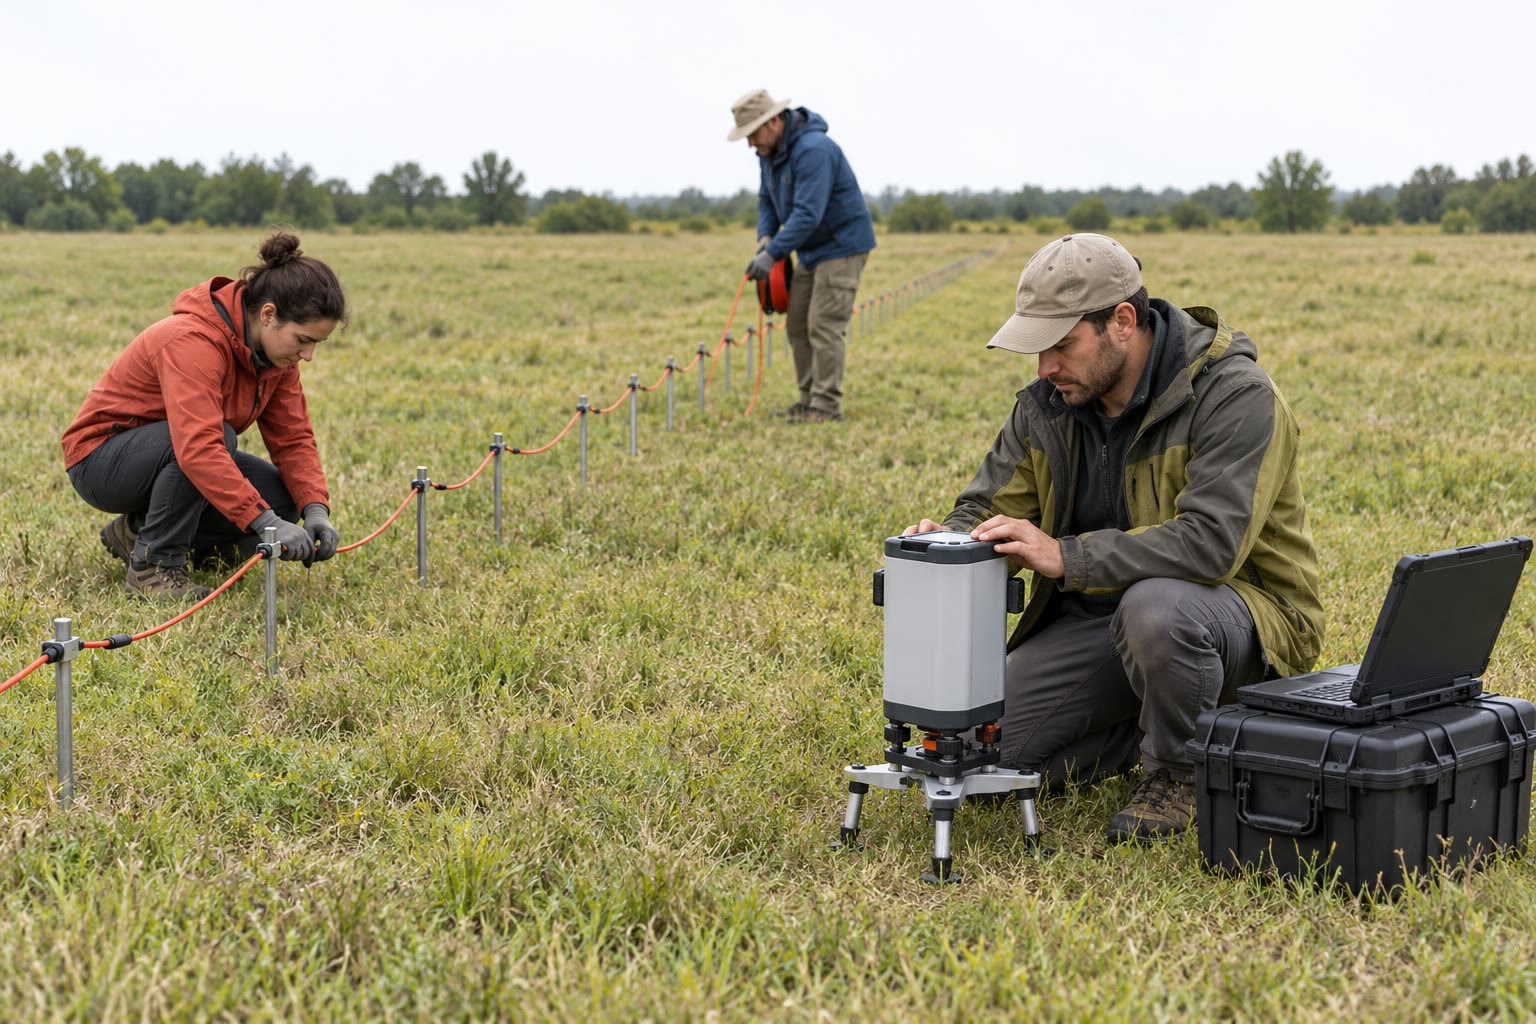
\includegraphics[width=\linewidth]{images/book5/ai/b3-geophysics-crew.jpg}

{\scriptsize Tim geofisika membentangkan kabel resistivitas, dengan sebuah
gravimeter di stasiun basisnya (ilustrasi buatan AI).}
\end{minipage}
\end{inthefield}

\begin{example}[Survei Varden]\label{ex:b3:field-lab-methods-3:varden}
Peta gravitasi menunjukkan minimum tertutup sekitar \qty{-2.3}{\milli\gal}
berpusat pada granit, memanjang utara--selatan: granit yang ringan
berlanjut di bawah penutup, dan paling panjang ke arah itu. Minimum
meluas hingga sekitar \qty{1}{km} dari singkapan, sehingga tubuh batuan melebar
seiring kedalaman. Setengah lebarnya memberi kedalaman awal untuk bola setara;
model dengan sisi vertikal dan dasar menunjukkan bahwa dasar antara satu
dan beberapa kilometer dalamnya menjelaskan puncak sama baiknya, dalam selisih beberapa
persepuluh miligal, sehingga dasar tetap tak diketahui---ketidakunikan
yang dibahas pada bagian sebelumnya. Di dasar lembah di atas granit,
sounding listrik dimulai pada resistivitas kerikil kering, turun di tempat
arus masuk ke aluvium jenuh air dan naik sepanjang garis lurus
berlereng satu: penutup konduktif di atas dasar yang sangat resistif, yaitu
granit, beberapa meter di bawah. Radar yang ditarik sepanjang dasar yang sama menunjukkan
gema datar pada sekitar \qty{20}{ns}: muka air tanah. Dan lintasan magnetik
melintasi sayap barat lipatan, tempat penutupnya tebal dan
sekis batuan dasar terletak sekitar dua ratus meter di bawah, mencatat
anomali tinggi simetris sekitar \qty{20}{nT} yang tidak dijelaskan peta mana pun: retas mafik,
kaya magnetit, terkubur di bawah penutup; jurusnya sepanjang
meridian magnetik itulah sebabnya anomalinya simetris. Para geofisikawan
melaporkannya sebagai retas dolerit yang terpotong pada ketidakselarasan, yang
disembunyikan penutup pada peta. Soal akhir pekan mengolah data
survei ini.
\end{example}
% ledger: gpg:susceptibility, gpg:resistivity, gpg:gpr-table

\section{Latihan}

\begin{exercise}[$\star$]\label{exo:b3:field-lab-methods-3:1}
(a)~Berapa bagian dari $g = \qty{9.81}{m.s^{-2}}$ yang setara dengan \qty{0.01}{\milli\gal}?
(b)~Seberapa jauh gravimeter harus dinaikkan agar pembacaannya
berubah sebesar \qty{0.01}{\milli\gal} semata-mata melalui efek udara-bebas? (c)~Melalui
efek udara-bebas dan Bouguer bersama-sama, dengan massa jenis
\qty{2670}{kg.m^{-3}}?
\end{exercise}

\begin{exercise}[$\star$]\label{exo:b3:field-lab-methods-3:2}
Sebuah bola berjari-jari \qty{50}{m} dan kontras massa jenis
\qty{+500}{kg.m^{-3}} dan pusatnya berada pada kedalaman \qty{100}{m}. Hitung
massa lebih, puncak anomalinya, dan setengah lebarnya $x_{1/2}$.
\end{exercise}

\begin{exercise}[$\star$]\label{exo:b3:field-lab-methods-3:3}
\omterm{def:b3:field-lab-methods-3:resistivity}{Susunan elektrode} Wenner dengan spasi $a = \qty{10}{m}$ menginjeksikan \qty{0.1}{A} dan
mengukur \qty{0.239}{V}. (a)~Hitung faktor geometri dan
\omterm{def:b3:field-lab-methods-3:resistivity}{resistivitas semu}. (b)~Tunjukkan bahwa susunan Schlumberger dengan $s =
\qty{15}{m}$ dan $l = \qty{5}{m}$ memiliki faktor geometri yang sama, dan
jelaskan mengapa.
\end{exercise}

\begin{exercise}[$\star$]\label{exo:b3:field-lab-methods-3:4}
Granit memiliki $\varepsilon_r = 5$. (a)~Hitung kecepatan radar. (b)~Sebuah
rekahan terletak \qty{10}{m} di bawah: hitung waktu bolak-balik gemanya.
(c)~Dengan $\sigma = \qty{1}{mS.m^{-1}}$, hitung kedalaman kulit dan
kedalaman berguna sekitar tiga kedalaman kulit. (d)~Bandingkan dengan lempung basah
yang memiliki $\varepsilon_r = 20$ dan $\sigma = \qty{10}{mS.m^{-1}}$.
\end{exercise}

\begin{exercise}[$\star\star$]\label{exo:b3:field-lab-methods-3:5}
(a)~Turunkan anomali silinder horizontal panjang berjari-jari $R$ dan
kontras massa jenis $\Delta\rho$, sumbunya berada pada kedalaman $z$, dari anomali
massa garis, dan tunjukkan bahwa $z = x_{1/2}$. (b)~Sebuah silinder dan sebuah bola
memberikan puncak yang sama dan setengah lebar yang sama $x_{1/2} = \qty{100}{m}$.
Bandingkan kedalaman keduanya. Interpretasi mana yang memberikan tubuh lebih dalam?
\end{exercise}

\begin{exercise}[$\star\star$]\label{exo:b3:field-lab-methods-3:6}
Anomali Bouguer dari model granit Varden, yang diambil setiap
\qty{100}{m} pada peta dengan \num{1120} titik yang meliputi $\qty{3.5}{km}
\times \qty{3.2}{km}$, berjumlah \qty{-438}{\milli\gal}. (a)~Terapkan
\cref{prop:b3:field-lab-methods-3:gauss} untuk menaksir defisit massa.
(b)~Defisit massa model adalah \qty{1.74e11}{kg}. Berapa pecahan yang
dapat ditangkap peta, dan di mana sisanya?
\end{exercise}

\begin{exercise}[$\star\star$]\label{exo:b3:field-lab-methods-3:7}
(a)~Retas tipis memiliki bagian atas \qty{30}{m} di bawah permukaan. Dengan aturan tiga
pembacaan per setengah lebar, dengan setengah lebar adalah lebar penuh
anomali pada setengah puncaknya, berapa spasi stasiun yang dibutuhkan? (b)~Lakukan hal yang sama
untuk puncak \qty{220}{m} di bawah permukaan. (c)~Mengapa satu survei tunggal tidak
dapat membedakan tubuh dangkal dan tubuh dalam sekaligus, kecuali dirancang untuk
yang dangkal?
\end{exercise}

\begin{exercise}[$\star\star$]\label{exo:b3:field-lab-methods-3:8}
Batu pasir yang jenuh air dengan resistivitas \qty{8}{\ohm\metre} memiliki
resistivitas \qty{80}{\ohm\metre}. (a)~Dengan $a = 1$ dan $m = 2$,
hitung porositasnya. (b)~Ulangi dengan $m = 1.8$ dan $m = 2.2$. Suku
mana dalam pengukuran yang mengendalikan ketidakpastian porositas?
\end{exercise}

\begin{exercise}[$\star\star$]\label{exo:b3:field-lab-methods-3:9}
(a)~Hitung tiga suku pertama deret dua lapisan dari
\cref{prop:b3:field-lab-methods-3:layers} pada $s = 2h_1$ untuk $k =
\num{0.5}$ dan $k = \num{-0.5}$, serta \omterm{def:b3:field-lab-methods-3:resistivity}{resistivitas semu} yang
dihasilkannya. (b)~Berapa limit $\rho_a/\rho_1$ untuk $s \ll h_1$ dan
$s \gg h_1$? (c)~Berapa rasio resistivitas $\rho_2/\rho_1$ yang sesuai dengan
$k = \pm 0.5$?
\end{exercise}

\begin{exercise}[$\star\star\star$]\label{exo:b3:field-lab-methods-3:10}
(a)~Turunkan faktor geometri susunan Wenner dari
\cref{thm:b3:field-lab-methods-3:point-source}. (b)~Turunkan pula faktor geometri
susunan Schlumberger, dan tunjukkan bahwa $\rho_a \to 2\pi s^2(-\mathrm{d}V/
\mathrm{d}r)/I$ saat $l/s \to 0$. (c)~Seberapa besar faktor pendekatan
$\pi s^2/(2l)$ melebihi nilai eksaknya ketika $l = s/10$?
\end{exercise}

\begin{exercise}[$\star\star\star$]\label{exo:b3:field-lab-methods-3:11}
Sebuah stasiun berada \qty{50}{m} di atas titik basis. Pembacaannya
\qty{0.01}{\milli\gal}, tingginya hingga \qty{5}{cm}; massa jenis
lempengan tidak pasti sebesar \qty{100}{kg.m^{-3}}, \omterm{def:b3:field-lab-methods-3:terrain}{koreksi medan} sebesar
\qty{0.2}{\milli\gal}. (a)~Susun anggaran galat anomali Bouguer
stasiun itu. (b)~Suku mana yang mendominasi, dan mana yang akan diperbaiki
untuk mendeteksi anomali \qty{0.1}{\milli\gal}? (c)~Berapa totalnya tanpa
suku \omterm{def:b3:field-lab-methods-3:terrain}{koreksi medan}?
\end{exercise}

\begin{exercise}[$\star\star\star$]\label{exo:b3:field-lab-methods-3:12}
Lima pembacaan gravitasi melintasi tubuh terkubur, pada $x = -600$, $-300$, $0$,
$300$ dan \qty{600}{m}, adalah \num{-0.69}, \num{-2.17}, \num{-4.16},
\num{-2.10} dan \qty{-0.73}{\milli\gal}, masing-masing dengan $\sigma =
\qty{0.03}{\milli\gal}$. (a)~Untuk model bola yang berpusat di bawah $x = 0$ pada
kedalaman \num{300}, \num{400} dan \qty{500}{m}, pilih massa yang
sesuai dengan pembacaan pusat, lalu hitung ketakcocokan $\chi^2$ masing-masing. (b)~Model mana
yang sesuai dengan data dalam galatnya? (c)~Bisakah tubuh berbentuk lain
sama cocoknya? Apa yang akan menentukan?
\end{exercise}

\section{Soal: Tubuh-tubuh tersembunyi di Perbukitan Varden}

\begin{problem}[{Soal akhir pekan --- reduksi survei Varden}]
\label{pb:b3:field-lab-methods-3:1}
Gunakan $G = \qty{6.674e-11}{m^3.kg^{-1}.s^{-2}}$, gradien udara-bebas
\qty{0.3086}{\milli\gal.m^{-1}} dan faktor Bouguer
\qty{0.1119}{\milli\gal.m^{-1}} (massa jenis \qty{2670}{kg.m^{-3}}).

\medskip\noindent\textbf{Bagian I --- Lintasan gravitasi tertutup.} Lintasan pada
profil gravitasi memberikan (pembacaan dalam miligal setelah kalibrasi, tinggi
dalam meter, waktu dalam jam setelah 09:00):
\begin{center}
\small
\begin{tabular}{lccccc}
\hline
stasiun & basis & \qty{3.0}{km} & \qty{3.5}{km} & \qty{4.0}{km} & basis \\
\hline
waktu & 0 & 0.5 & 0.9 & 1.3 & 2.0 \\
tinggi & 176.1 & 149.0 & 145.5 & 158.0 & 176.1 \\
pembacaan & 2846.512 & 2851.075 & 2850.497 & 2849.392 & 2846.708 \\
\hline
\end{tabular}
\end{center}
\begin{enumerate}
\item Hitung laju hanyutan lintasan tersebut.
\item Koreksi ketiga pembacaan stasiun terhadap hanyutan dan nyatakan
  relatif terhadap basis.
\item Terapkan koreksi udara-bebas dan koreksi Bouguer untuk selisih
  tinggi, dan nyatakan anomali Bouguer tiap stasiun relatif terhadap
  basis.
\item \omterm{def:b3:field-lab-methods-3:gravimeter}{Hanyutan instrumen} saja adalah \qty{0.040}{\milli\gal.h^{-1}}.
  Apa penyebab sisa perubahan di basis, dan mengapa itu dapat
  dihilangkan bersama hanyutan?
\item Model tempat pembacaan berasal memberikan ketiga anomali
  relatif terhadap basis sebagai \num{-0.825}, \num{-2.131} dan
  \qty{-0.825}{\milli\gal}. Hitung galat reduksi. Tinggi
  pada tabel dibulatkan hingga \qty{0.1}{m}: galat apa yang dapat ditimbulkan
  pembulatan ini, dan apakah itu menjelaskan galatnya?
\item Ketelitian tinggi yang bagaimana menjaga anomali tereduksi dalam
  \qty{0.01}{\milli\gal}? Mengapa panduan survei meminta
  \qty{3.3}{cm}, angka yang lebih ketat?
\end{enumerate}

\medskip\noindent\textbf{Bagian II --- Anomali granit.} Sepanjang
profil, anomali mencapai minimum \qty{-2.293}{\milli\gal}, pada
$x = \qty{3.50}{km}$, dan memotong setengah nilai itu pada $x = 3.048$ dan
\qty{3.952}{km}. Model granit memiliki kontras massa jenis
\qty{-130}{kg.m^{-3}}, dan permukaan tanah di pusat berada pada \qty{145.5}{m}
di atas permukaan laut.
\begin{enumerate}[resume]
\item Hitung lebar setengah $x_{1/2}$ dan kedalaman pusat
  bola ekuivalen.
\item Hitung defisit massa bola itu, dan jari-jarinya untuk
  kontras massa jenis granit. Apa yang janggal pada hasilnya?
\item Pusat massa model berada \qty{864}{m} di bawah permukaan tanah dan
  defisit massanya \qty{1.74e11}{kg}. Mengapa aturan lebar setengah memberi
  tubuh yang lebih dangkal dan lebih ringan?
\item Silinder vertikal dengan luas yang sama seperti granit pada
  ketidakselarasan memiliki jari-jari \qty{461}{m}. Hitung anomalinya pada sumbu
  untuk puncak di permukaan tanah dan dasar pada kedalaman \qty{1645}{m}, dan untuk
  kedalaman tak terhingga.
\item Temukan, dengan coba-coba atau dengan menyelesaikan persamaan, kedalaman dasar yang membuat silinder ini
  memberikan anomali teramati \qty{-2.29}{\milli\gal}.
\item Hitung anomali silinder dengan puncaknya \qty{6}{m} di bawah
  (dasar \qty{1645}{m}). Dapatkah gravitasi menunjukkan apakah granit mencapai
  permukaan di bawah aluvium?
\end{enumerate}

\medskip\noindent\textbf{Bagian III --- Dasar lembah.} Sounding Schlumberger
pada dasar lembah di atas granit memberikan (jarak setengah $s$ dalam
meter, $\rho_a$ dalam \unit{\ohm\metre}):
\begin{center}
\small
\begin{tabular}{lcccccccc}
\hline
$s$ & 1 & 2 & 4 & 6 & 10 & 20 & 30 & 40 \\
$\rho_a$ & 577 & 526 & 387 & 350 & 449 & 821 & 1309 & 1684 \\
\hline
\end{tabular}
\end{center}
Pada profil radar sepanjang dasar yang sama, sebuah pipa menghasilkan hiperbola dengan
puncaknya pada \qty{10.7}{ns} dan waktu \qty{17.1}{ns} sejauh \qty{1}{m}
di samping; gema datar tiba pada \qty{20.0}{ns}.
\begin{enumerate}[resume]
\item Pada $s = \qty{20}{m}$, MN panjangnya \qty{2}{m} dan arus
  \qty{50}{mA}. Hitung faktor geometri dan beda potensial yang terukur.
\item Hitung kecepatan radar, permitivitas relatif
  aluvium, dan kedalaman pipa.
\item Gema datar itu adalah muka air tanah. Seberapa dalam letaknya?
\item Taksir konduktansi $S$ aluvium dari pembacaan pada
  20, 30 dan \qty{40}{m}.
\item Aluvium kering memiliki \qty{600}{\ohm\metre}, dan aluvium jenuh
  \qty{222}{\ohm\metre}. Hitung ketebalan aluvium jenuh
  dan kedalaman puncak granit. Apakah taksiran ini tinggi
  atau rendah, dan mengapa?
\item Air tanah memiliki \qty{20}{\ohm\metre}. Hitung porositas
  aluvium dengan \omterm{prop:b3:field-lab-methods-3:archie}{hukum Archie} untuk $m = 2$, dan rentang bagi $m$
  antara \num{1.3} dan \num{2.8}.
\end{enumerate}

\medskip\noindent\textbf{Bagian IV --- Lintasan magnetik.} Lintasan itu membentang
ke timur dari $x = \qty{1.70}{km}$, satu stasiun setiap \qty{50}{m} dan setiap
dua menit; stasiun basis mencatat pada menit yang sama. Pembacaan
itu, setelah dikurangi \qty{48000}{nT}, adalah:
\begin{center}
\small
\setlength{\tabcolsep}{3.5pt}
\begin{tabular}{lccccccccccc}
\hline
$x$ (km) & 1.70 & 1.75 & 1.80 & 1.85 & 1.90 & 1.95 & 2.00 & 2.05 & 2.10 & 2.15 & 2.20 \\
lintasan & 3.4 & 4.8 & 6.3 & 8.1 & 10.3 & 12.8 & 15.8 & 19.2 & 22.9 & 26.2 & 28.0 \\
basis & 0.0 & 0.7 & 1.5 & 2.2 & 2.9 & 3.6 & 4.3 & 5.0 & 5.7 & 6.4 & 7.0 \\
\hline
$x$ (km) & 2.25 & 2.30 & 2.35 & 2.40 & 2.45 & 2.50 & 2.55 & 2.60 & 2.65 & 2.70 & \\
lintasan & 27.7 & 25.8 & 23.3 & 20.9 & 19.0 & 17.6 & 16.6 & 15.9 & 15.5 & 15.2 & \\
basis & 7.6 & 8.2 & 8.8 & 9.4 & 9.9 & 10.4 & 10.9 & 11.3 & 11.7 & 12.1 & \\
\hline
\end{tabular}
\end{center}
Medan utama adalah \qty{48000}{nT}, dengan inklinasi \ang{65}.
\begin{enumerate}[resume]
\item Terapkan \omterm{def:b3:field-lab-methods-3:magnetic}{koreksi diurnal} dan berikan anomali terkoreksi pada
  setiap stasiun.
\item Tunjukkan bahwa tanpa koreksi, anomali tidak pernah turun hingga setengah
  puncaknya di sisi timur.
\item Tentukan puncak dan dua titik tempat anomali terkoreksi bernilai setengah
  puncaknya, dengan interpolasi linear, lalu hitung lebar setengah-puncak.
\item Anomali itu simetris. Apa artinya itu bagi jurus
  benda tersebut, dan jenis benda seperti apa yang diasumsikan oleh aturan lebar setengah-puncak?
\item Hitung hasil kali $\kappa t$ antara suseptibilitas dan ketebalan.
  Jika retas itu berupa dolerit dengan suseptibilitas \num{0.03}, seberapa tebal
  retas itu?
\item Apakah stasiunnya cukup rapat?
\item Berikan kedalaman ke puncak retas tersembunyi di bawah tanah, hingga
  sepuluh meter terdekat, dan bandingkan dengan kedalaman ketidakselarasan
  pada model geologi wilayah itu, \qty{222}{m} di
  titik ini.
\end{enumerate}
\end{problem}
% ledger: gpg:grav-survey, gpg:mag-field, keys:archie
